\documentclass[final]{article}
\usepackage[paperwidth=48in,paperheight=48in,margin=0.55in]{geometry}
\usepackage{graphicx}
\usepackage{xcolor}
\usepackage{booktabs}
\usepackage{array}
\usepackage{amsmath}
\usepackage{tikz}
\usepackage{hyperref}
\usepackage{lmodern}
\usepackage{microtype}
\usepackage{enumitem}

\pagestyle{empty}
\setlength{\parindent}{0pt}
\setlength{\parskip}{0.035in}
\setlength{\fboxsep}{0.07in}
\setlength{\fboxrule}{1.1pt}
\setlist[itemize]{leftmargin=0.24in,itemsep=0.012in,topsep=0.01in}

\definecolor{posterbg}{HTML}{F5F0E8}
\definecolor{posterink}{HTML}{1F2523}
\definecolor{posterprimary}{HTML}{245447}
\definecolor{posteraccent}{HTML}{B85C38}
\definecolor{postersage}{HTML}{8EA898}
\definecolor{posterline}{HTML}{A99985}
\definecolor{posterpanel}{HTML}{FFFCF7}

\pagecolor{posterbg}
\hypersetup{colorlinks=true,urlcolor=posterprimary}

\newcounter{posterfigure}
\newcounter{postertable}

\newcommand{\bodytext}{\fontsize{16.4}{19.5}\selectfont}
\newcommand{\smalltext}{\fontsize{11.8}{14.0}\selectfont}
\newcommand{\captionfont}{\fontsize{10.8}{12.9}\selectfont}
\newcommand{\paneltitle}[1]{%
  {\fontsize{24}{28}\selectfont\bfseries\color{posterprimary}#1}\par
  \vspace{0.015in}{\color{posteraccent}\rule{\linewidth}{0.03in}}\vspace{0.03in}
  \bodytext
}
\newcommand{\panelbox}[2]{%
  \fcolorbox{posterline}{posterpanel}{%
    \begin{minipage}[t]{0.965\linewidth}
    \paneltitle{#1}
    #2
    \end{minipage}%
  }%
}
\newcommand{\figcaption}[1]{%
  \refstepcounter{posterfigure}%
  \par{\captionfont\color{posterink}\textbf{Figure \theposterfigure.} #1\par}%
}
\newcommand{\tabcaption}[1]{%
  \refstepcounter{postertable}%
  {\captionfont\color{posterink}\textbf{Table \thepostertable.} #1\par}%
  \vspace{0.025in}%
}
\newcommand{\metric}[2]{%
  \begin{minipage}[t]{0.30\linewidth}
  \centering
  {\fontsize{31}{35}\selectfont\bfseries\color{posteraccent}#1}\par
  {\smalltext #2}
  \end{minipage}
}

\begin{document}
\bodytext

\begin{center}
{\fontsize{45}{50}\selectfont\bfseries\color{posterprimary}Toward Substrate-Agnostic SERS Classification Using Siamese Metric Learning}\par
\vspace{0.055in}
{\fontsize{21}{25}\selectfont\bfseries\color{posterink}Jesse Levine$^{1}$, Hal Bowen-Smith$^{1}$, Greg Wardle$^{1}$, and Dr. Li-Lin Tay$^{1}$}\par
\vspace{0.02in}
{\fontsize{15.5}{19}\selectfont\color{posterink}$^{1}$Metrology Research Centre, National Research Council Canada, Ottawa, ON, Canada}
\end{center}

\vspace{0.04in}
{\color{posterprimary}\rule{\linewidth}{0.07in}}
\vspace{0.015in}

\begin{center}
\metric{98.76\%}{Stage 1 chemical-substrate pair one-shot accuracy on 403 query spectra}
\hfill
\metric{97.5\%}{Stage 2 chemical-label accuracy under leave-one-substrate-family-out testing}
\hfill
\metric{0.837}{Chemical-label organization gain over substrate-family organization in embedding space}
\end{center}

\vspace{0.035in}

\begin{minipage}[t]{0.49\linewidth}
\panelbox{1. Background / Motivation}{%
SERS spectra carry two signals at once: the \textbf{chemical analyte} and the \textbf{enhancing substrate}. The original model learned this combined signature well, but that is not the same as recognizing the chemical independently of the substrate.

\textbf{Starting point:} classify measured chemical-substrate pairs such as \texttt{4np\_\_AgNP} or \texttt{pyridine\_\_PICO}.

\textbf{Current target:} classify only the chemical label, while holding out an entire substrate family during training. This is the stricter test because the model cannot directly memorize spectra from the held-out surface.

\textbf{Central question:} can a Siamese encoder learn an embedding where spectra from the same chemical are close together even when the substrate changes?

\vspace{0.05in}
\begin{center}
\resizebox{0.78\linewidth}{!}{%
\begin{tikzpicture}[x=1in,y=1in]
\node[draw=posterline,fill=posterpanel,rounded corners=0.12in,minimum width=3.65in,minimum height=0.84in,align=center,line width=1.3pt] (s1) at (0,0) {\textbf{Substrates}\\Commercial PICO, pSERS\\Printed Ag/Au nanoparticle paper};
\node[draw=posterline,fill=posterpanel,rounded corners=0.12in,minimum width=3.65in,minimum height=0.84in,align=center,line width=1.3pt] (s2) at (4.3,0) {\textbf{Analyte exposure}\\Soak in diluted analyte\\solution for 1 h};
\node[draw=posterline,fill=posterpanel,rounded corners=0.12in,minimum width=3.65in,minimum height=0.84in,align=center,line width=1.3pt] (s3) at (8.6,0) {\textbf{Dry}\\Allow substrate to dry\\before measurement};
\node[draw=posterline,fill=posterpanel,rounded corners=0.12in,minimum width=3.65in,minimum height=0.84in,align=center,line width=1.3pt] (s4) at (12.9,0) {\textbf{SERS spectrum}\\Raw intensity vs.\\Raman shift};
\draw[->,line width=2.2pt,color=posterprimary] (s1) -- (s2);
\draw[->,line width=2.2pt,color=posterprimary] (s2) -- (s3);
\draw[->,line width=2.2pt,color=posterprimary] (s3) -- (s4);
\end{tikzpicture}%
}
\end{center}
\figcaption{Sample-preparation workflow used for the SERS measurements. Commercial PICO and pSERS sensors are used alongside in-house printed Ag/Au nanoparticle-paper substrates; each analyte-substrate preparation is soaked, dried, and measured as a raw Raman-shift spectrum before preprocessing.}
}
\end{minipage}
\hfill
\begin{minipage}[t]{0.49\linewidth}
\panelbox{2. Samples / Dataset Matrix}{%
The available data are structured as a chemical-by-substrate-family matrix. After grouping AgNP with Ag and AuNP with Au, benzenethiol and pyridine span all four substrate families, while 4NP is missing on Au because it does not respond there.

\begin{center}
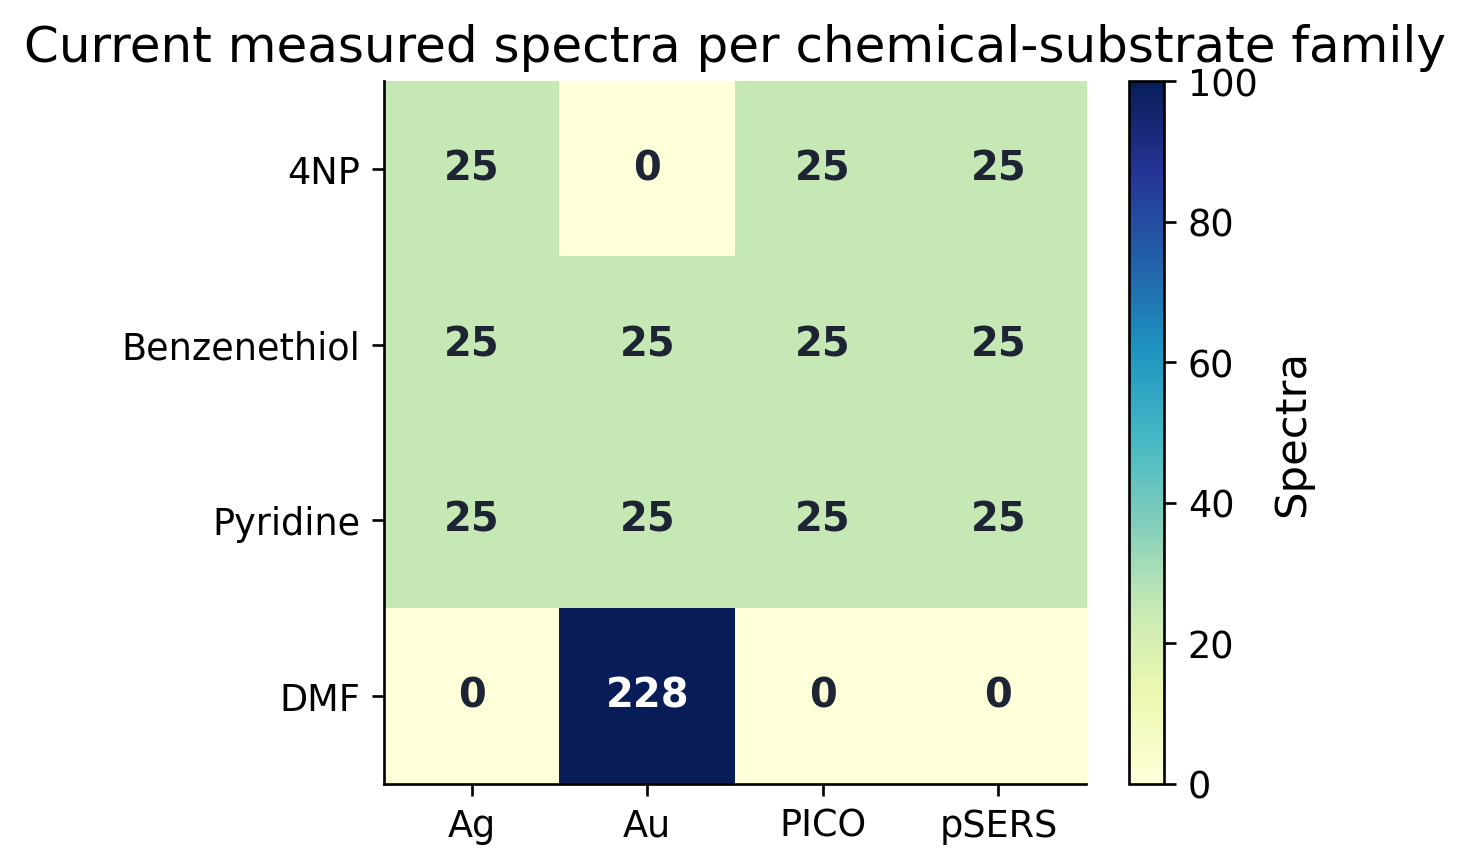
\includegraphics[width=0.42\linewidth]{figures/dataset_matrix_heatmap.png}
\end{center}
\figcaption{Current measured spectra per chemical-substrate family after grouping equivalent metal substrates. Numbers inside cells are spectra counts. The substrate-agnostic model uses 4NP, benzenethiol, and pyridine; DMF is excluded from the transfer model because it is measured only on Au and therefore cannot support cross-substrate chemical learning.}

\textbf{Dataset implication:} the task is not merely low-sample classification. The matrix is also structurally incomplete: one chemical is missing on one substrate family and only three chemicals are available for the substrate-agnostic target. This makes leave-one-substrate-family-out testing informative but still limited.
}
\end{minipage}

\vspace{0.08in}

\begin{minipage}[t]{0.49\linewidth}
\panelbox{3. Chemical-Substrate Classification}{%
The first successful model used the same general Siamese idea, but the predicted class was the \textbf{chemical-substrate pair}. This is useful for recognizing known measurement conditions, but it does not prove substrate-agnostic chemical recognition.

\tabcaption{Stage 1 pair-classification model. This model learned pair identities, so strong performance means the network recognized combined chemical-surface signatures rather than chemical identity alone.}
\begin{center}
\smalltext
\begin{tabular}{p{0.31\linewidth}p{0.58\linewidth}}
\toprule
\textbf{Item} & \textbf{Original pair model} \\
\midrule
Target & Chemical-substrate pair identity \\
Encoder & Shared Conv1D Siamese encoder, 64-D L2-normalized embedding \\
Loss & Contrastive loss, margin 1.0 \\
Inference & One known reference spectrum per pair class \\
Result & 98.76\% top-1 accuracy on 403 query spectra \\
\bottomrule
\end{tabular}
\end{center}

\begin{center}
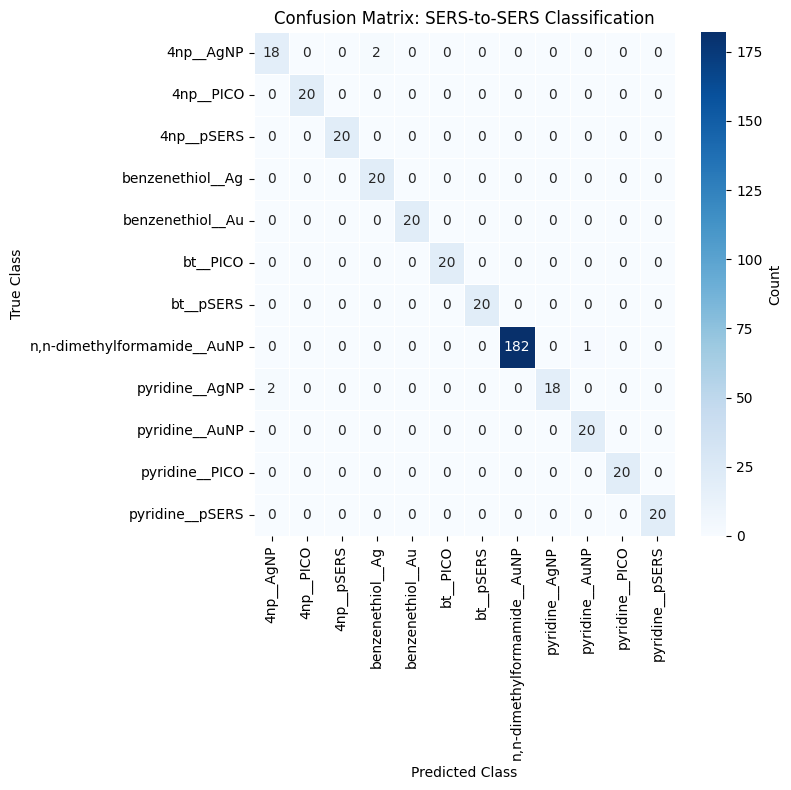
\includegraphics[width=0.45\linewidth]{figures/pair_classifier_confusion_matrix_notebook.png}
\end{center}
\figcaption{Original notebook confusion matrix for SERS-to-SERS chemical-substrate pair classification. The strong diagonal shows that most pair labels are recovered correctly, but each class still encodes the substrate. This result motivated the next step: keep the Siamese metric-learning strategy, but change the label from pair identity to chemical identity.}
}
\end{minipage}
\hfill
\begin{minipage}[t]{0.49\linewidth}
\panelbox{4. Substrate-Agnostic Siamese Model}{%
\begin{minipage}[t]{0.51\linewidth}
\tabcaption{Current model input and training setup. Table captions are placed above tables; the encoder input is the processed first-derivative spectrum, not raw intensity.}
\begin{center}
\smalltext
\begin{tabular}{p{0.32\linewidth}p{0.58\linewidth}}
\toprule
\textbf{Step} & \textbf{Role} \\
\midrule
Crop 330.906--1797.919 cm$^{-1}$ & Remove low-wavenumber device artifact region. \\
SNV normalization & Reduce intensity and offset variation. \\
Savitzky-Golay first derivative & Emphasize peak shape/position and suppress broad background. \\
Row L2 normalization & Put spectra on a comparable metric-learning scale. \\
Conv1D encoder & 1$\rightarrow$16 conv, ReLU, pool; 16$\rightarrow$32 conv, ReLU, pool; flatten; linear/ReLU to 64-D; L2-normalized embedding. \\
Training & Triplet loss, margin 0.2; Adam $10^{-3}$; batch size 32; 100 epochs; noise/shift augmentation; GPU/CUDA required. \\
\bottomrule
\end{tabular}
\end{center}
\end{minipage}
\hfill
\begin{minipage}[t]{0.45\linewidth}
\begin{center}
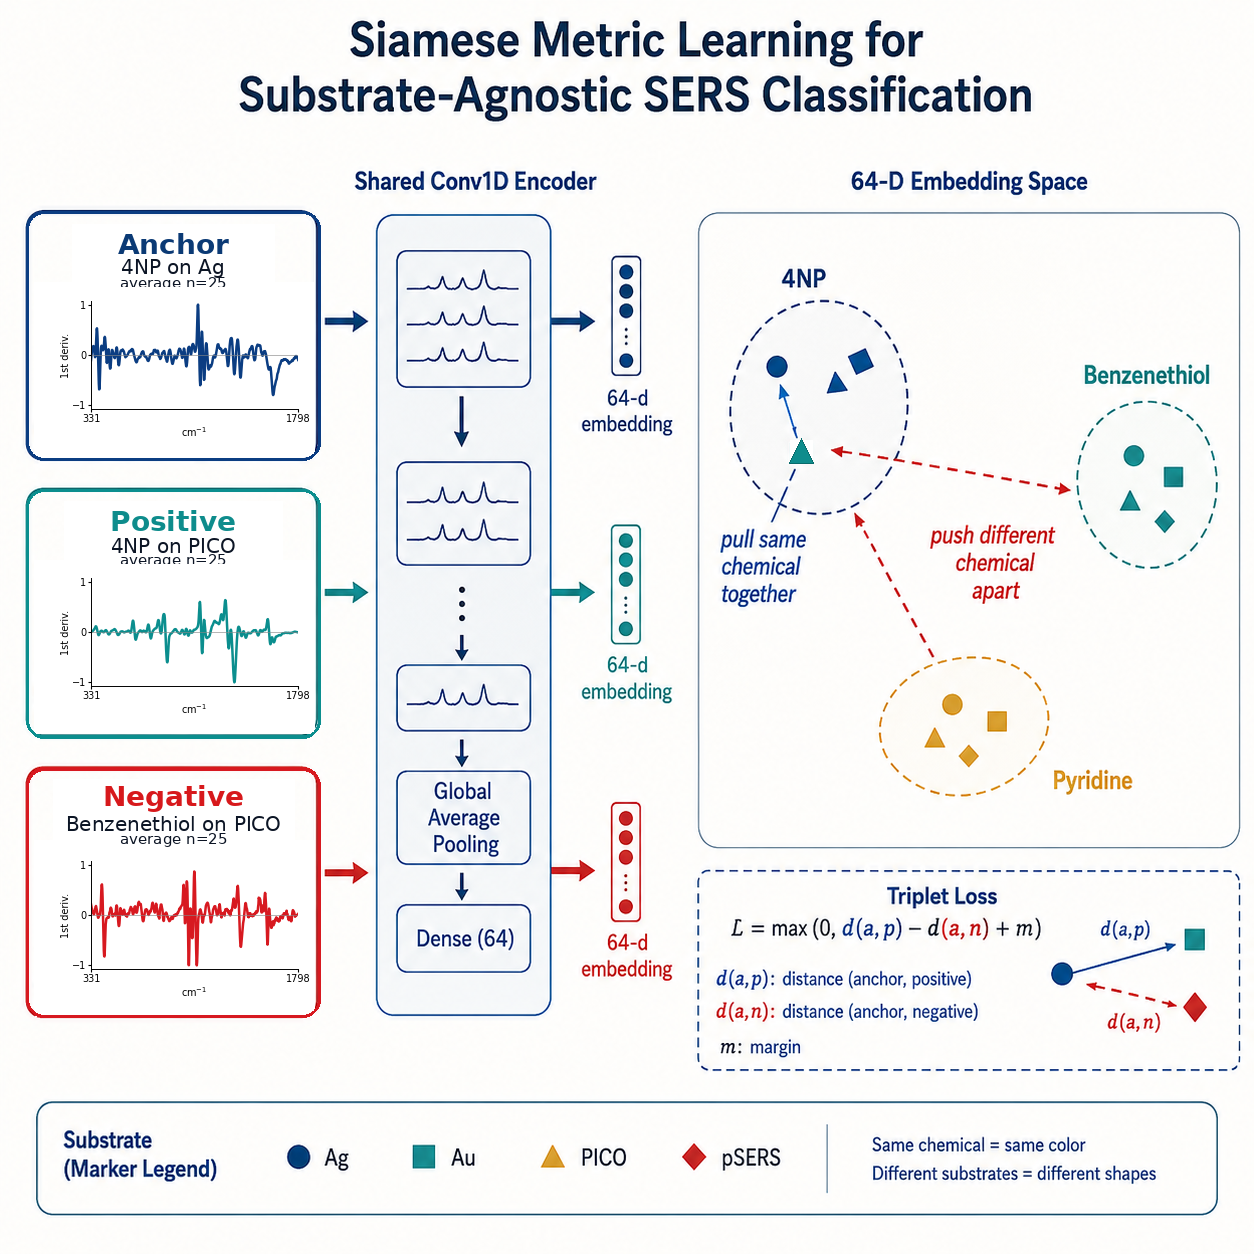
\includegraphics[width=0.64\linewidth]{figures/siamese_metric_learning_4np_pico_positive_average.png}
\end{center}
\figcaption{Siamese/triplet-learning schematic. Anchor and positive spectra share the same chemical label and are pulled together; the negative has a different chemical label and is pushed away. The spectra drawn at left are mean raw spectra for interpretability only. The actual encoder input is the cropped, SNV-normalized, first-derivative, L2-normalized spectrum.}
\end{minipage}

\vspace{0.045in}
\begin{minipage}[t]{0.37\linewidth}
\tabcaption{Leave-one-substrate-family-out performance for the best substrate-agnostic Siamese model. The fair fold-level score uses only chemicals present in the held-out substrate family.}
\begin{center}
\smalltext
\begin{tabular}{lrr}
\toprule
\textbf{Held out} & \textbf{Acc.} & \textbf{True-label F1} \\
\midrule
Ag & 0.920 & 0.919 \\
Au & 0.980 & 0.990 \\
PICO & 1.000 & 1.000 \\
pSERS & 1.000 & 1.000 \\
\bottomrule
\end{tabular}
\end{center}
\end{minipage}
\hfill
\begin{minipage}[t]{0.59\linewidth}
\begin{center}
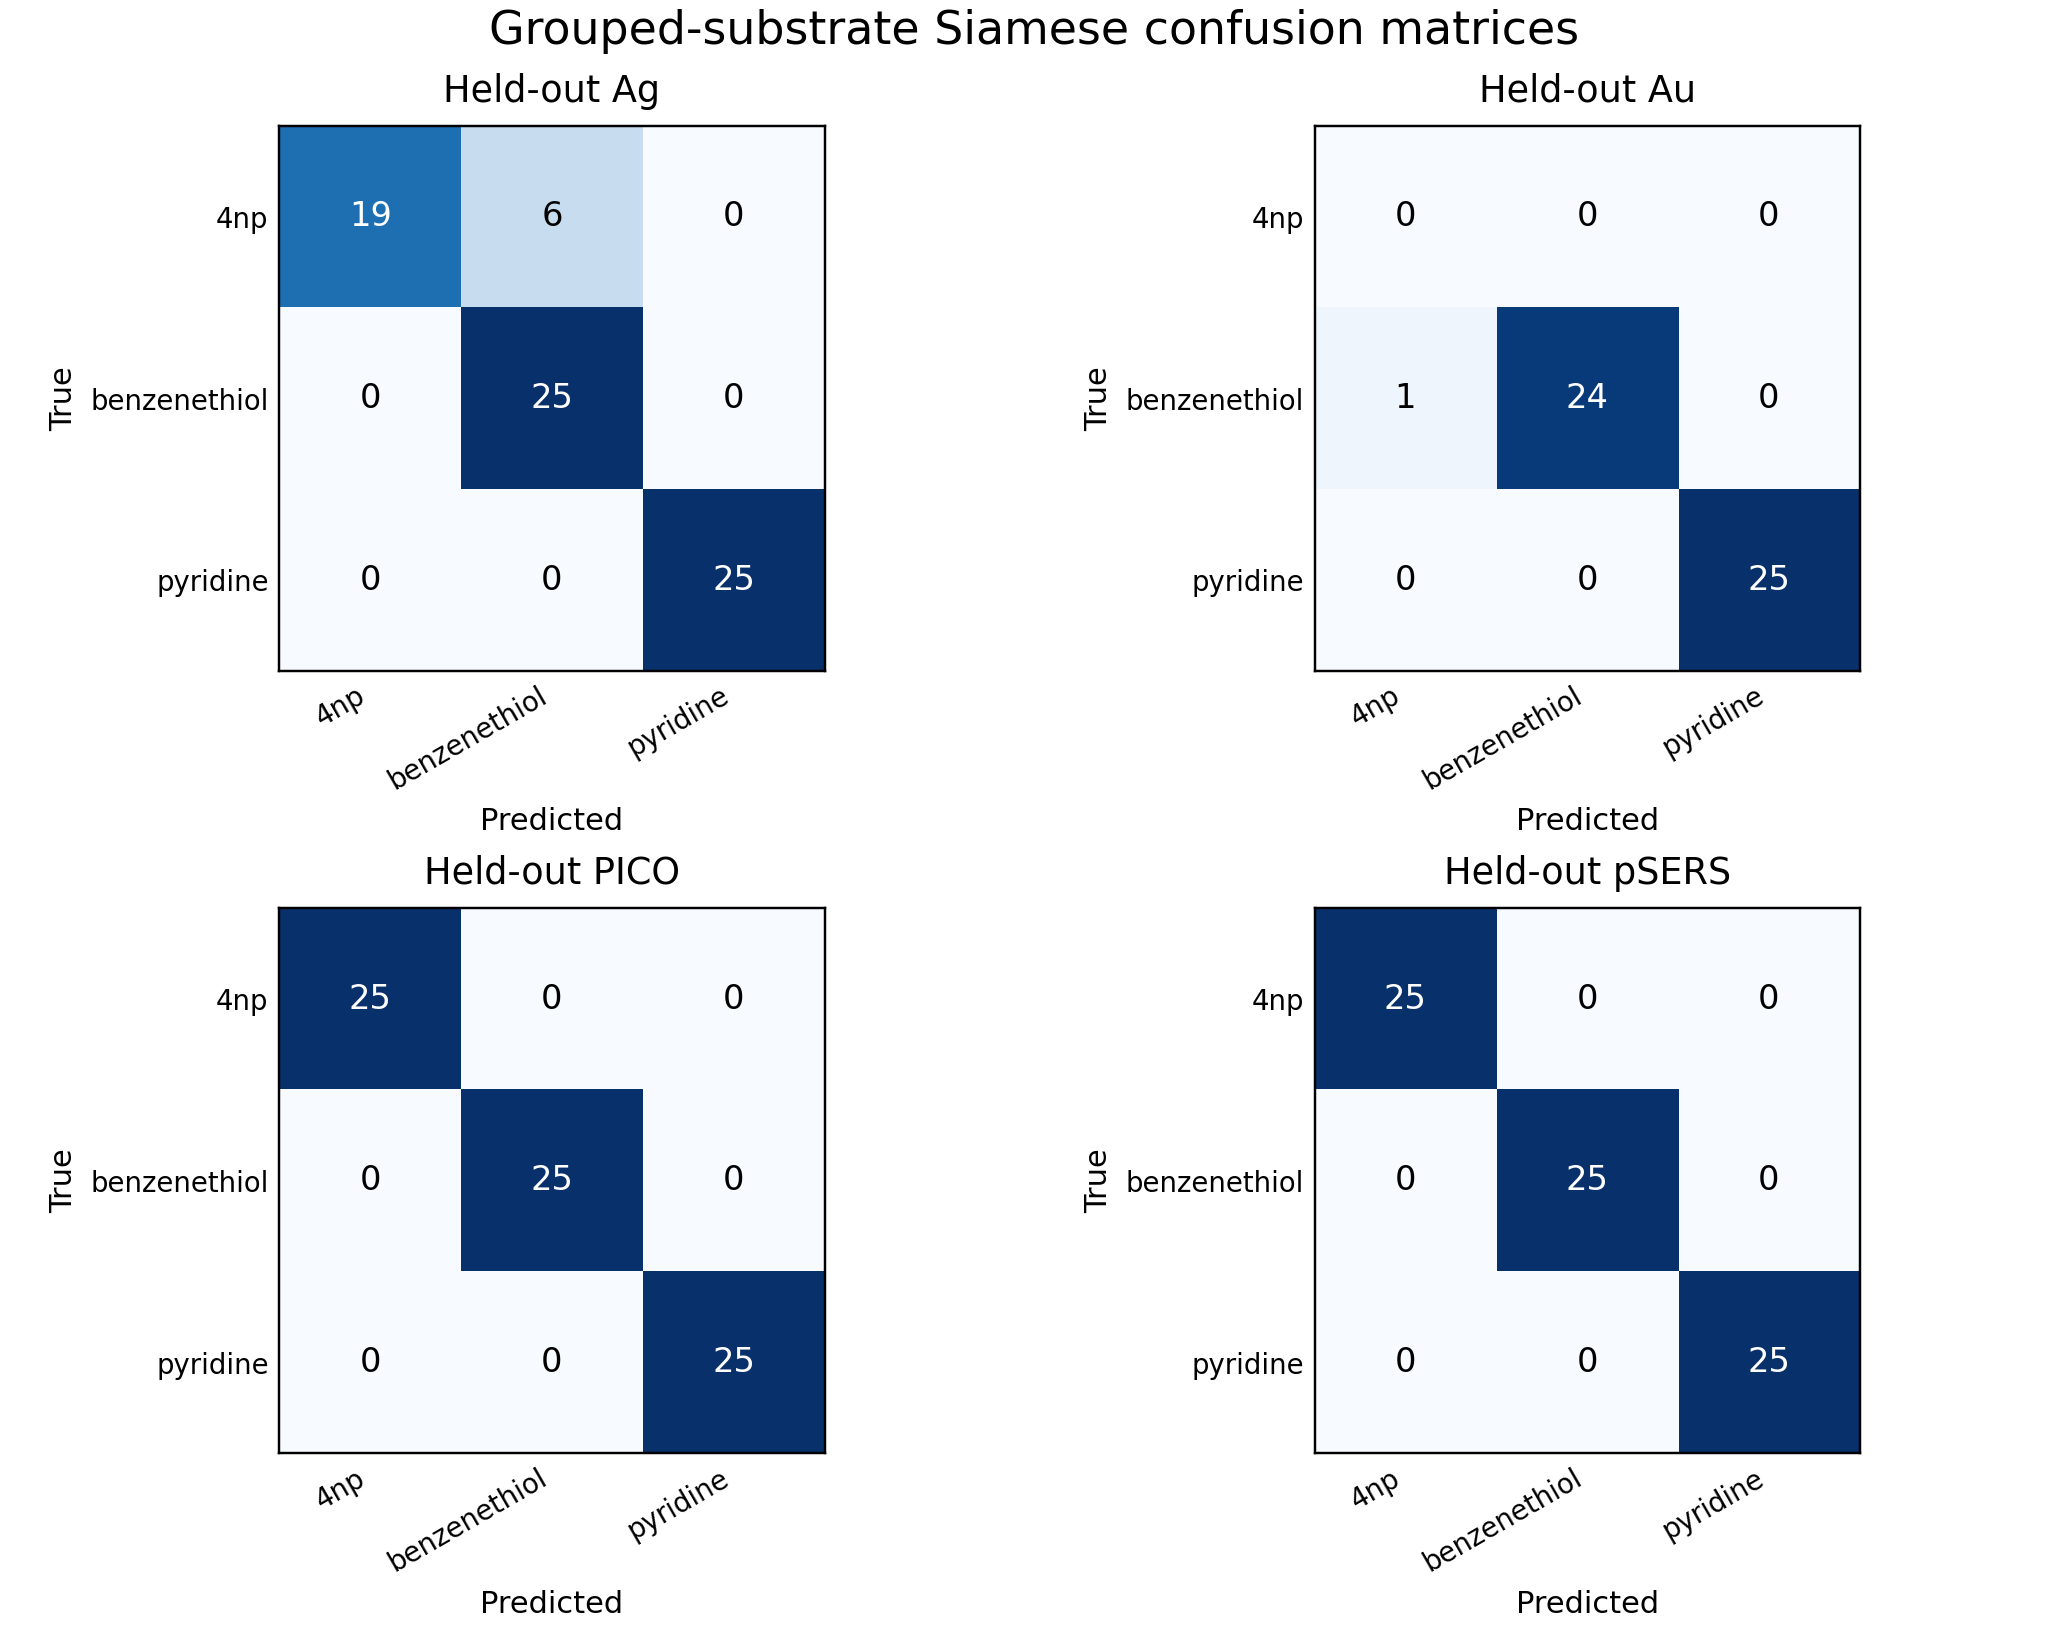
\includegraphics[width=0.62\linewidth]{../sers_substrate_agnostic_supervisor_report/figures/grouped_best_confusions.png}
\end{center}
\figcaption{Grouped-substrate Siamese confusion matrices. The model transfers cleanly to PICO and pSERS. The main residual failure is the held-out Ag fold, where 6/25 4NP spectra are predicted as benzenethiol; this is the clearest weak point for future data collection.}
\end{minipage}
}
\end{minipage}

\vspace{0.08in}

\panelbox{5. Geometry, Takeaways, And Future Directions}{%
\begin{minipage}[t]{0.64\linewidth}
\begin{center}
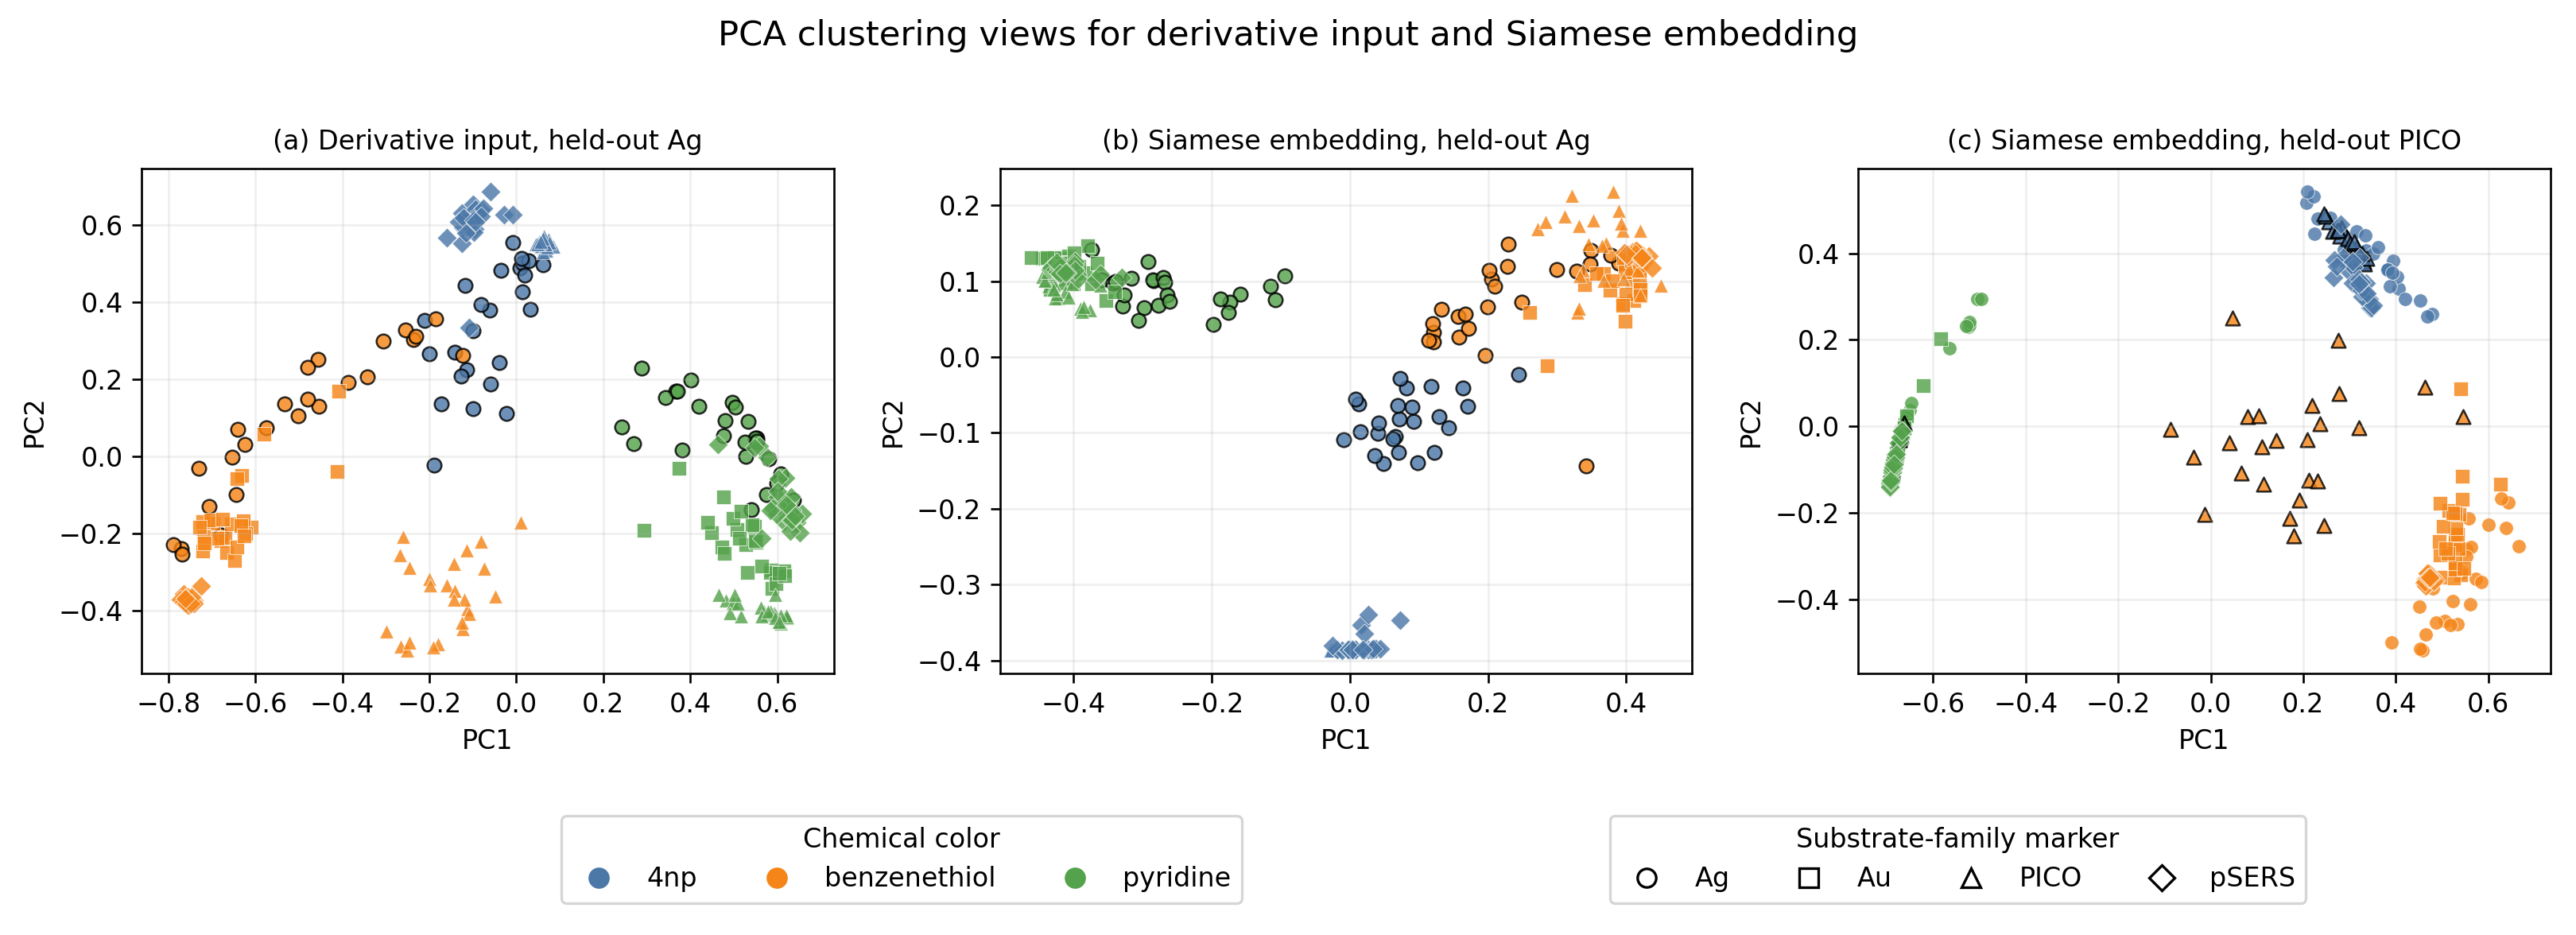
\includegraphics[width=\linewidth]{../sers_substrate_agnostic_supervisor_report/figures/combined_pca_clustering.png}
\end{center}
\figcaption{PCA views comparing the derivative-input space and the learned Siamese embedding. Chemical identity is shown by color and substrate family by marker shape. In derivative space, chemical and substrate effects are partially entangled. In embedding space, same-chemical spectra become tighter and more separable, while substrate-family structure is reduced. The remaining Ag/4NP weakness is visible as a local overlap rather than a complete failure of chemical organization.}
\end{minipage}
\hfill
\begin{minipage}[t]{0.33\linewidth}
\tabcaption{Silhouette analysis of the representation geometry. A higher chemical silhouette and lower substrate silhouette means spectra are organized more by chemical identity than by substrate family.}
\begin{center}
\smalltext
\begin{tabular}{lrrr}
\toprule
\textbf{Representation} & \textbf{Chem. sil.} & \textbf{Substrate sil.} & \textbf{Diff.} \\
\midrule
Derivative input & 0.304 & 0.101 & 0.203 \\
Siamese embedding & 0.797 & -0.040 & 0.837 \\
\bottomrule
\end{tabular}
\end{center}

\textbf{Takeaways}
\begin{itemize}
\item The original model solved chemical-substrate pair recognition; the substrate was still part of the class label.
\item The current model keeps the Siamese metric-learning strategy but changes the target to chemical identity and the evaluation to leave-one-substrate-family-out transfer.
\item The embedding generally pulls same-chemical spectra closer and reduces substrate-family organization.
\item The weak point is specific: 4NP transfer to held-out Ag, not a uniform collapse across substrates.
\end{itemize}

\textbf{Future directions}
\begin{itemize}
\item Fill the chemical-by-substrate matrix with more responsive chemicals measured on every substrate family.
\item Add independent preparations, measurement days, and map locations, not only repeated spectra from the same preparation.
\item Prioritize Ag-family 4NP and benzenethiol measurements to determine whether the residual confusion is chemical overlap, substrate-specific enhancement, or insufficient coverage of preparation variability.
\item Validate on a truly new substrate or new acquisition day after the matrix is expanded.
\end{itemize}
\end{minipage}
}

\vfill
{\color{posterprimary}\rule{\linewidth}{0.05in}}\par
\vspace{0.05in}
\hfill
\begin{minipage}[b]{0.36\linewidth}
\fcolorbox{posterline}{posterpanel}{%
  \begin{minipage}{0.96\linewidth}
  {\fontsize{22}{26}\selectfont\bfseries\color{posterprimary}Acknowledgments}\par
  \vspace{0.04in}
  {\smalltext This work was carried out at the NRC Metrology Research Centre and prepared for the Canadian Societies for Chemistry and Chemical Engineering 2026 Conferences and Exhibition (x2026).}\par
  \vspace{0.08in}
  \begin{center}
  
\includegraphics[width=0.48\linewidth]{figures/logos/nrc_logo.png}
  \end{center}
  \end{minipage}%
}
\end{minipage}

\end{document}
